\documentclass[12pt, letterpaper]{article}
\usepackage[toc,page]{appendix}
\usepackage[utf8]{inputenc}
\usepackage[pdftex]{graphicx}
\usepackage{xspace}
\usepackage[stable]{footmisc}
\usepackage{hyperref}
\usepackage{fullpage}
\usepackage{subcaption}
\usepackage{placeins}
\hypersetup{
    colorlinks=true,
    linkcolor=blue,
    filecolor=magenta,
    urlcolor=cyan,
}
\graphicspath{ {/home/tobiasjenegger/Documents/summary/} }
\title{GLAD analysis}
\author{Tobias Jenegger}
\date{}
\begin{document}
\begin{titlepage}
\maketitle
\end{titlepage}
\section{RUNS used for calibration = SWEEP RUNS without target}

\begin{center}
    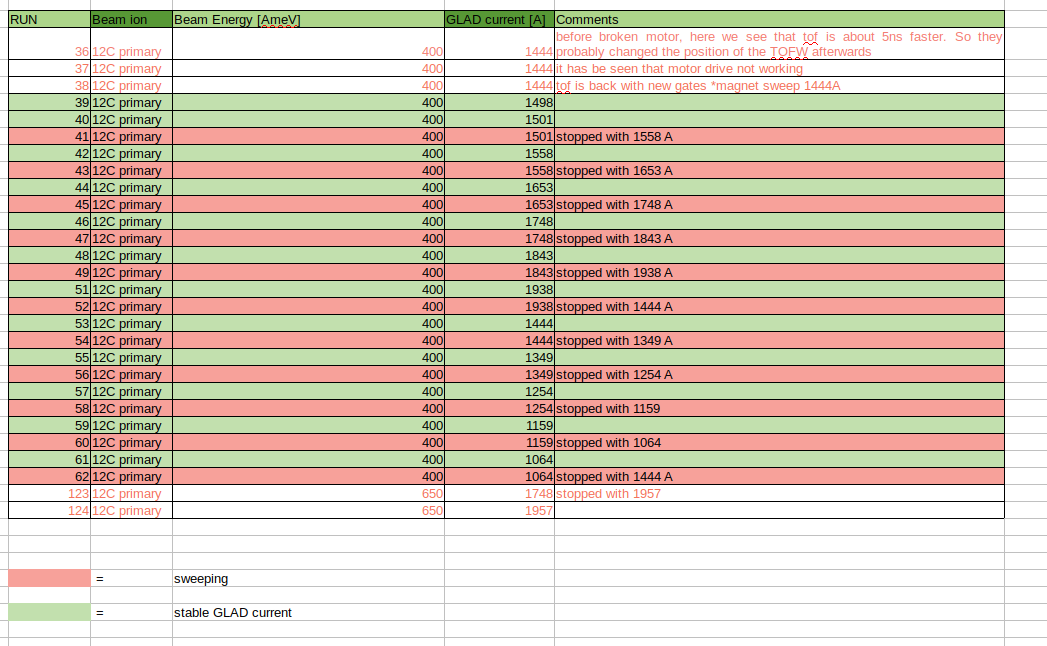
\includegraphics[width=1.0\textwidth]{runs_screenshot.png}
\end{center}
Run 62 could not be used to compare with RUN 53 (1444A), as the GLAD current was sweeping continuously from 1064 to 1444 Ampere.
\begin{figure}[!htbp]
\begin{subfigure}{.5\textwidth}
	\centering
	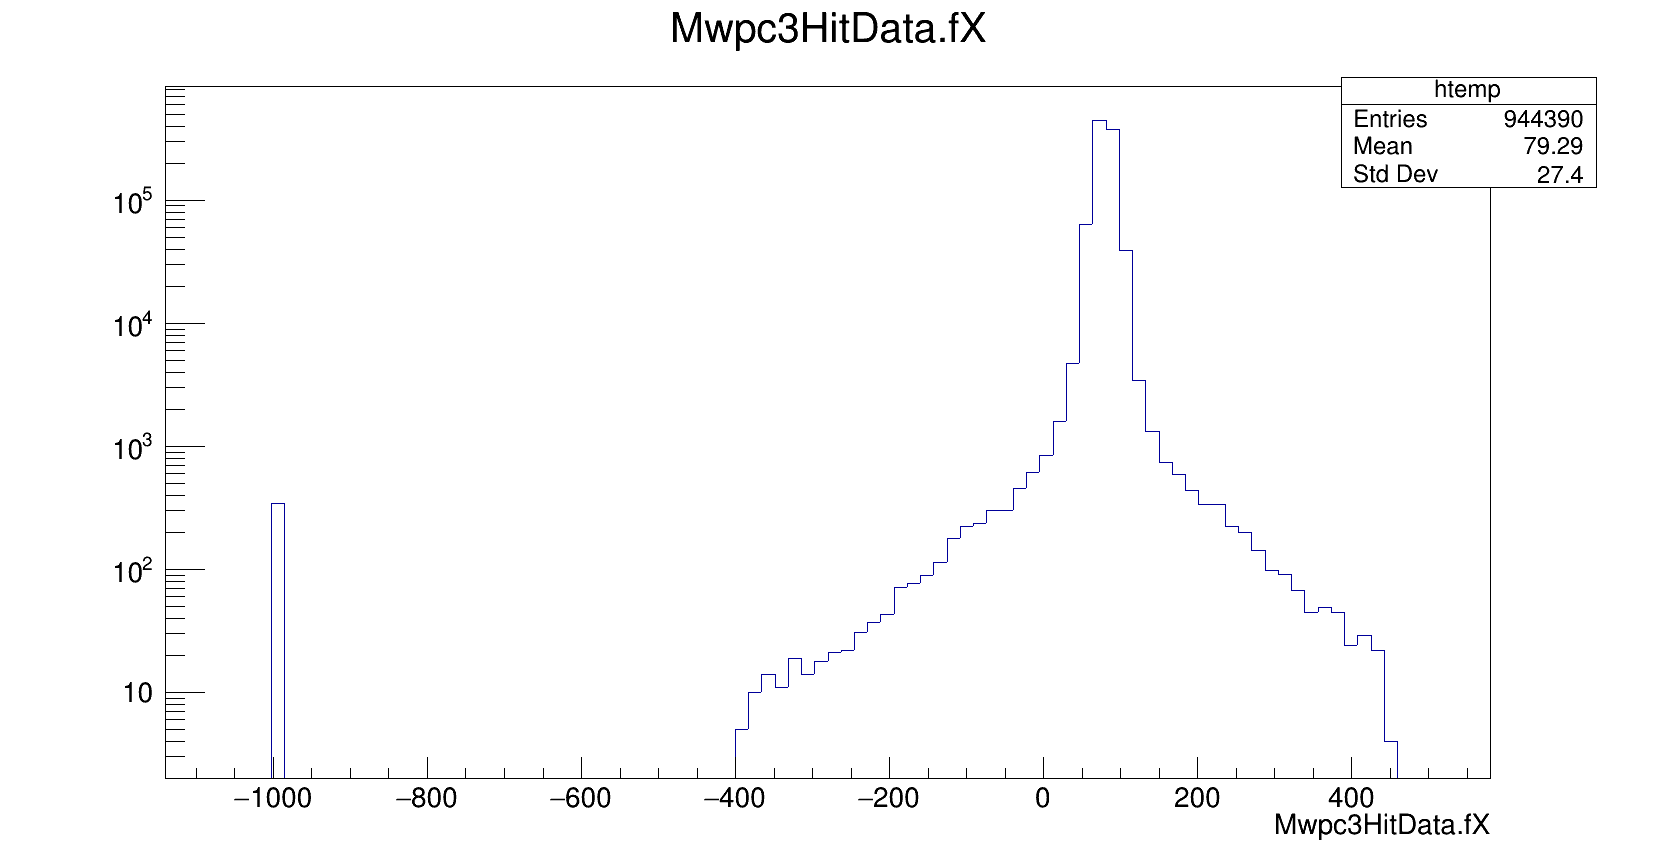
\includegraphics[width=.9\linewidth]{run53_mw3.png}
	\caption{"Event counts for MWPC3.fX in RUN 53 with GLAD current 1444A."}
	\label{fig:sub-second}
\end{subfigure}	
\begin{subfigure}{.5\textwidth}
	\centering
	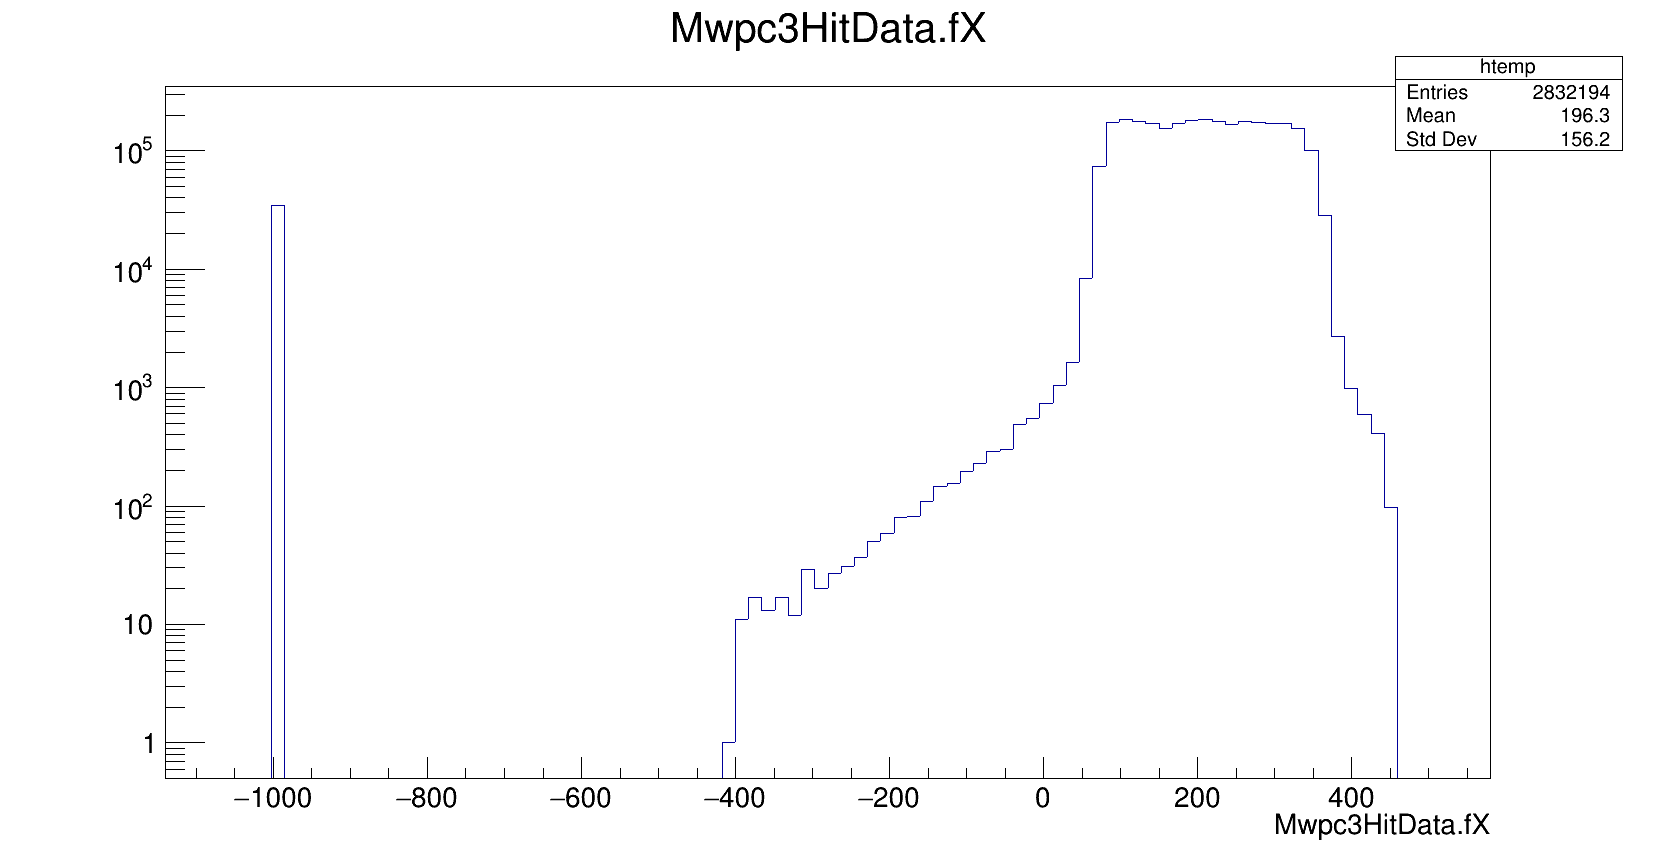
\includegraphics[width=.9\linewidth]{run62_mw3.png}
	\caption{"Event counts for MWPC3.fX in RUN 62 with sweeping GLAD current."}
	\label{fig:sub-second}
\end{subfigure}
\end{figure}
\begin{figure}[!htbp]
\begin{subfigure}{.9\textwidth}
	\centering
	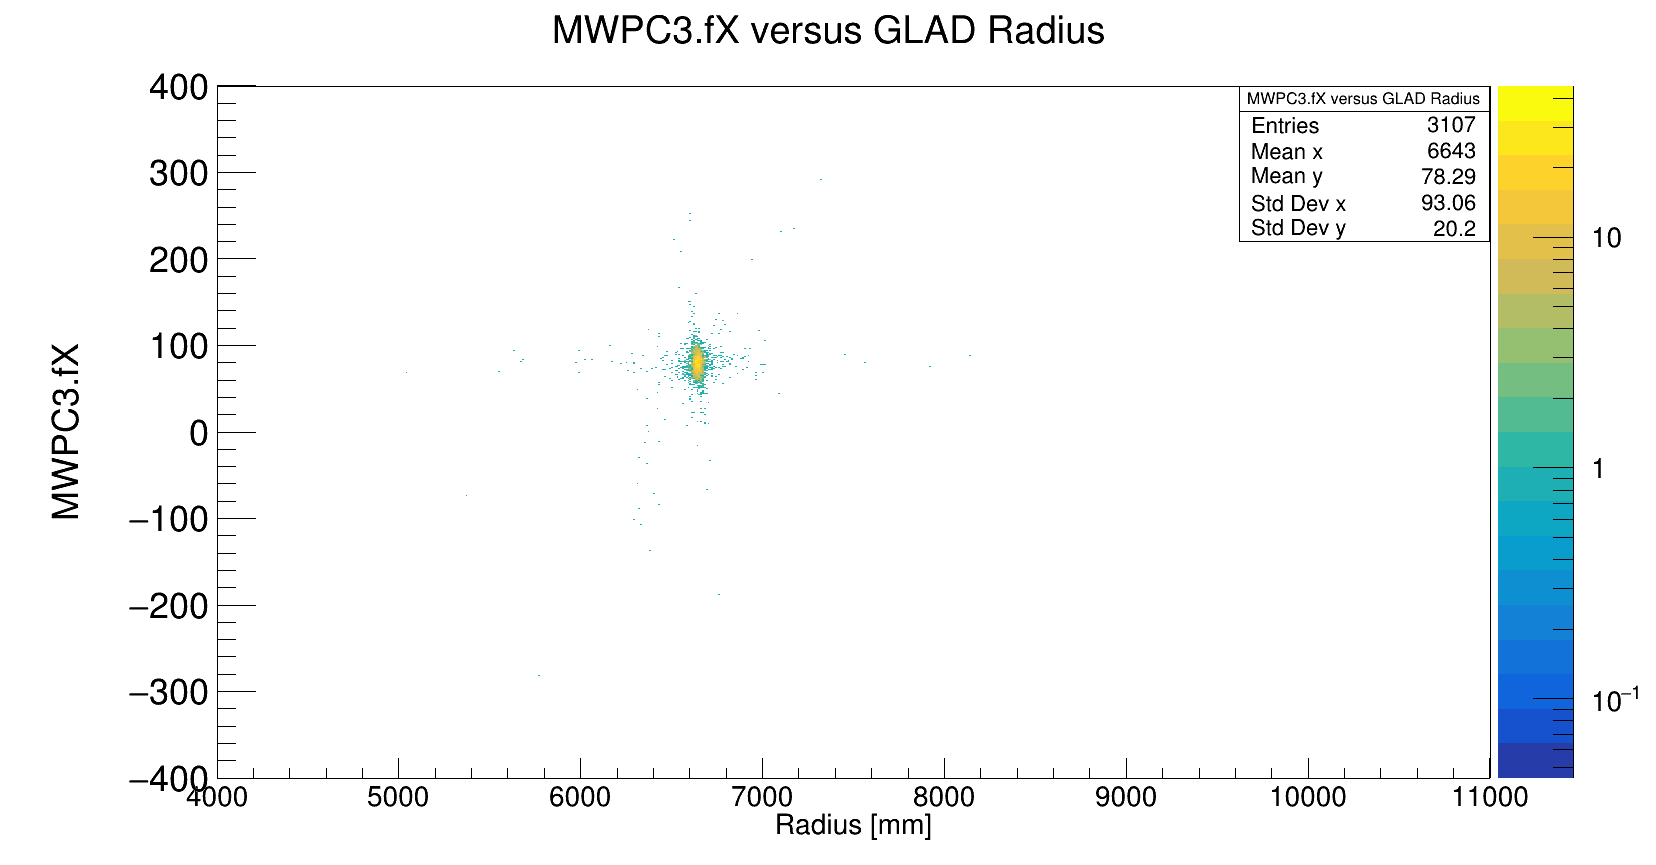
\includegraphics[width=.9\linewidth]{mw3_vs_rad_run53.png}
	\caption{"Radius vs MWPC3.fX for RUN 53 with GLAD current 1444A."}
	\label{fig:sub-second}
\end{subfigure}	
\begin{subfigure}{.9\textwidth}
	\centering
	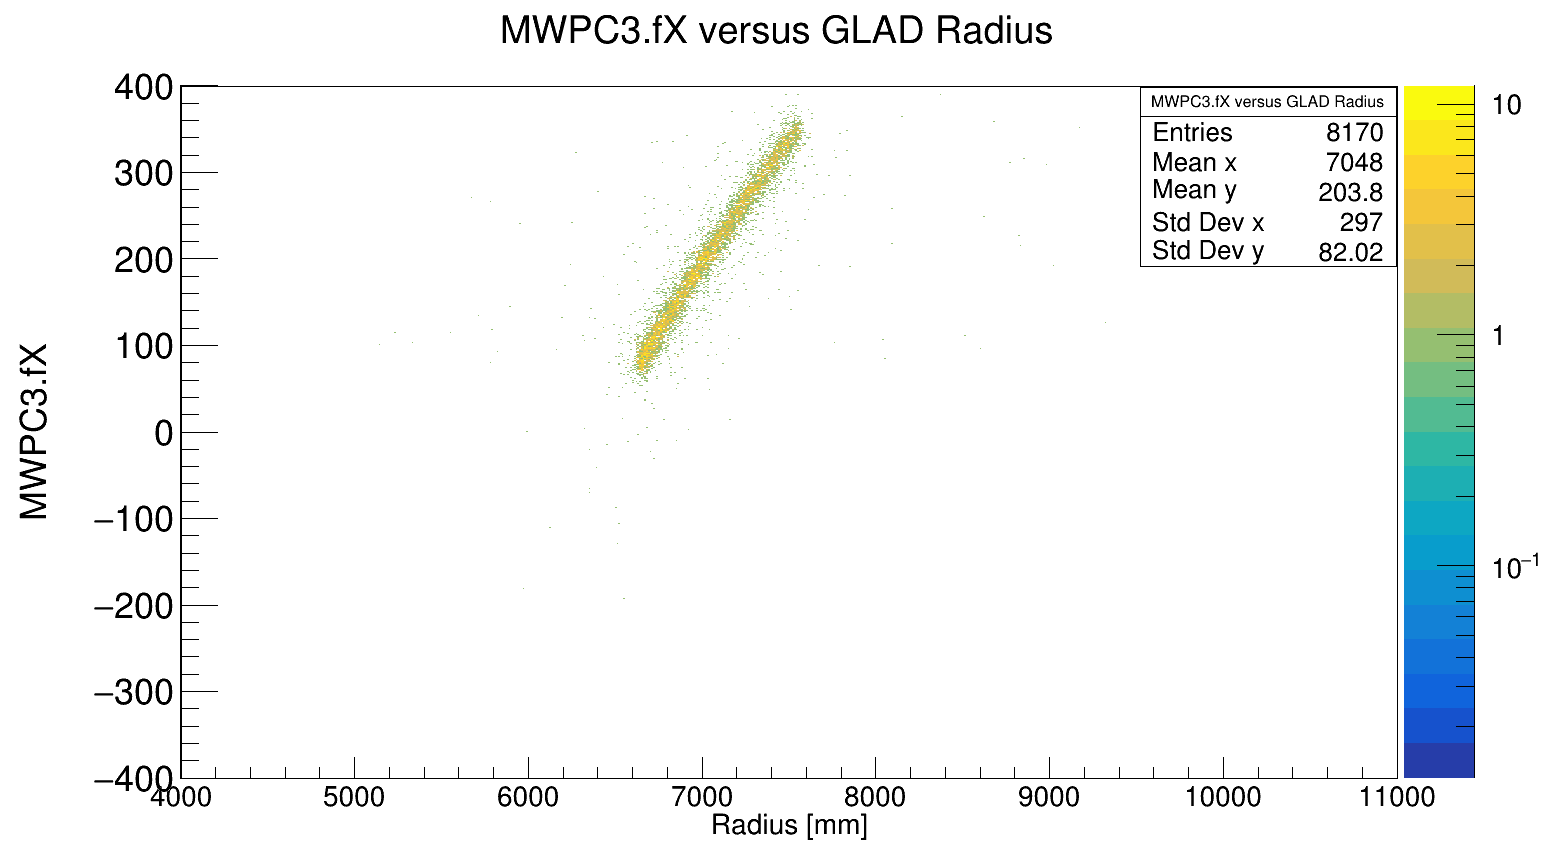
\includegraphics[width=.9\linewidth]{mw3_vs_rad_62.png}
	\caption{"Radius vs MWPC3.fX for RUN 62 with sweeping GLAD current."}
	\label{fig:sub-second}
\end{subfigure}
\end{figure}

Taking sweep RUNS 39-61 we get following plot for B-Field versus Current (where the B-Field is calculated from given Brho divided by the calculated mean radius for given current):\\
\begin{figure}[!htbp]
	\centering
	\includegraphics[width=.9\linewidth]{scale_glad.png}
	\caption{"Current vs B-Field using the E-Log Entry for RUN39, I = 1498."}
\end{figure}
\\
As the GLAD current can just be tuned in multiple steps of 19A, the Current value for RUN 39 falls out of the range. Most probably that was a typo. Making same plot but changing the Current number of RUN 39 to 1482 Ampere we get:\\
\begin{figure}[!htbp]
	\centering
	\includegraphics[width=.9\linewidth]{scale_glad_corr.png}
	\caption{"Current vs B-Field, setting I = 1482 for RUN39."}
\end{figure}
\\
Using as current 1482 for RUN 39 we get from the linear fit going through (0,0) as slope $k = 0.000657193$ (with B $= k \cdot I$). From the proportional fitting line we see that for ramping up the data points lie slightly below the fitting line but then for ramping down slowly above the line. This indicated pattern could be due to the  supposed underlying magnetic remanence which adds a positive offset when ramping down. \\
Plotting $k = $ Brho/(rho$\cdot$ current) versus current we get the proportional factor $k$ for each RUN:\\

\begin{figure}[!htbp]
	\centering
	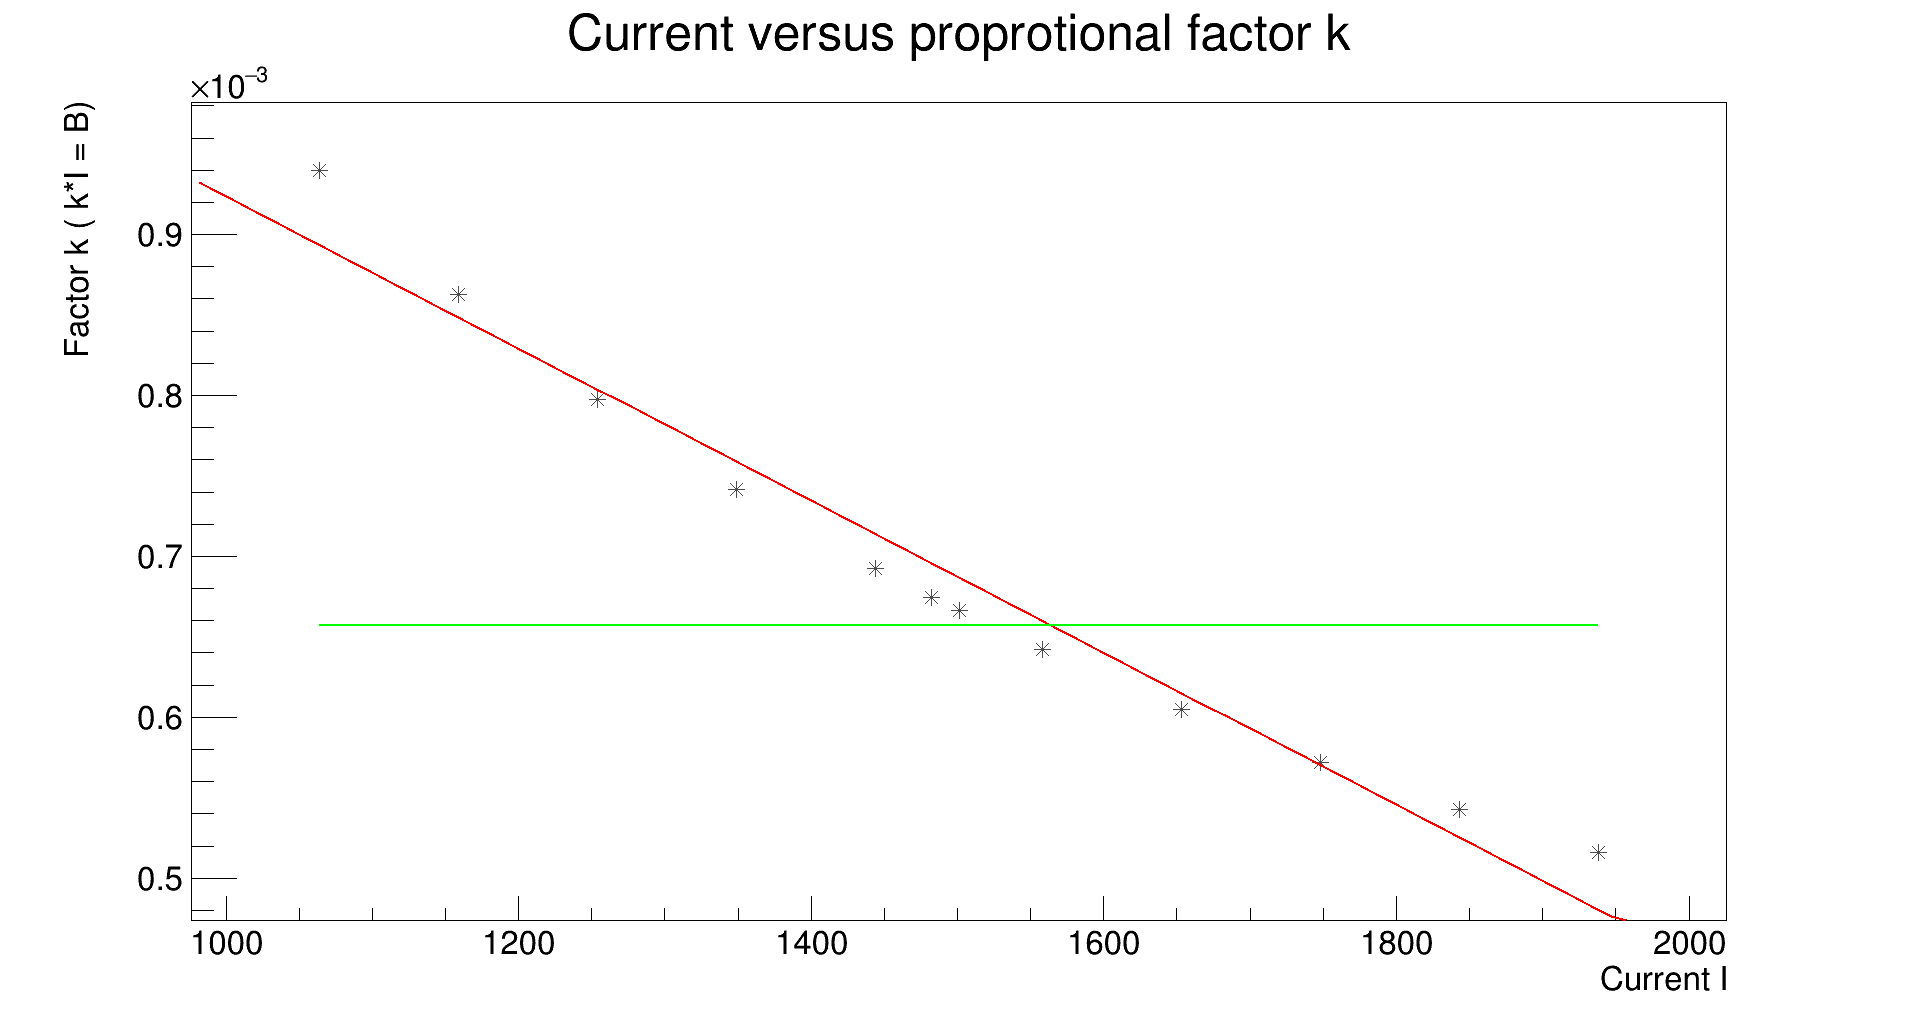
\includegraphics[width=.9\linewidth]{k_factor.png}
	\caption{"Current vs proportional factor $k$ for RUNs 39-61.Green line: $k$ value from fit B vs I; red line: Fit ax+b of $k$ vs I"}
	\label{fig:k_vs_i}
\end{figure}

The plot in figure \ref{fig:k_vs_i} shows decreasing $k$ values for increasing current. The green line in figure \ref{fig:k_vs_i} shows the $k$ value retrieved from the proportional fit of B-Field versus current. The red line in figure \ref{fig:k_vs_i} is a linear fit (ax+b) of the values in the plot.\\
From the fit we get follwing values for a and b:\\
\begin{itemize}
\item a $= -4.72574e-07$
\item b $= 0.00139628$
\item $\chi/NDf = 6.03242e-09/10$
\end{itemize}

As it can be seen the data points deviate noticeable from the straight fitting line. That means not just second order terms, but third and higher terms need to be considered when describing the B-Field by the current. \\
From figure \ref{fig:k_vs_i} it can also be read off the value of the slope for the respective current. As $k$ (i.e. the slope) decreases with increasing current, the curve flattens out for higher current values. This is also the case in a hysteresis curve.\\
When fitting the datapoints of $k$ with a polynomial of second order ($ax^{2}+bx +c$) we get the fitting curve shown in figure \ref{fig:k_vs_i_pol2} with the parameters:\\
\begin{itemize}
\item a $= 3.22629e-10$
\item b $= -1.44161e-06$
\item c $= 0.00210266$
\item $\chi/NDf = 1.3088e-10/9$
\end{itemize}
It can be clearly seen that the fit in figure \ref{fig:k_vs_i_pol2} is much better than in figure \ref{fig:k_vs_i} (see also the $\chi/NDf$ values). Hence the B-Field can be described well by third order terms in I (curent).
\begin{figure}[!htbp]
	\centering
	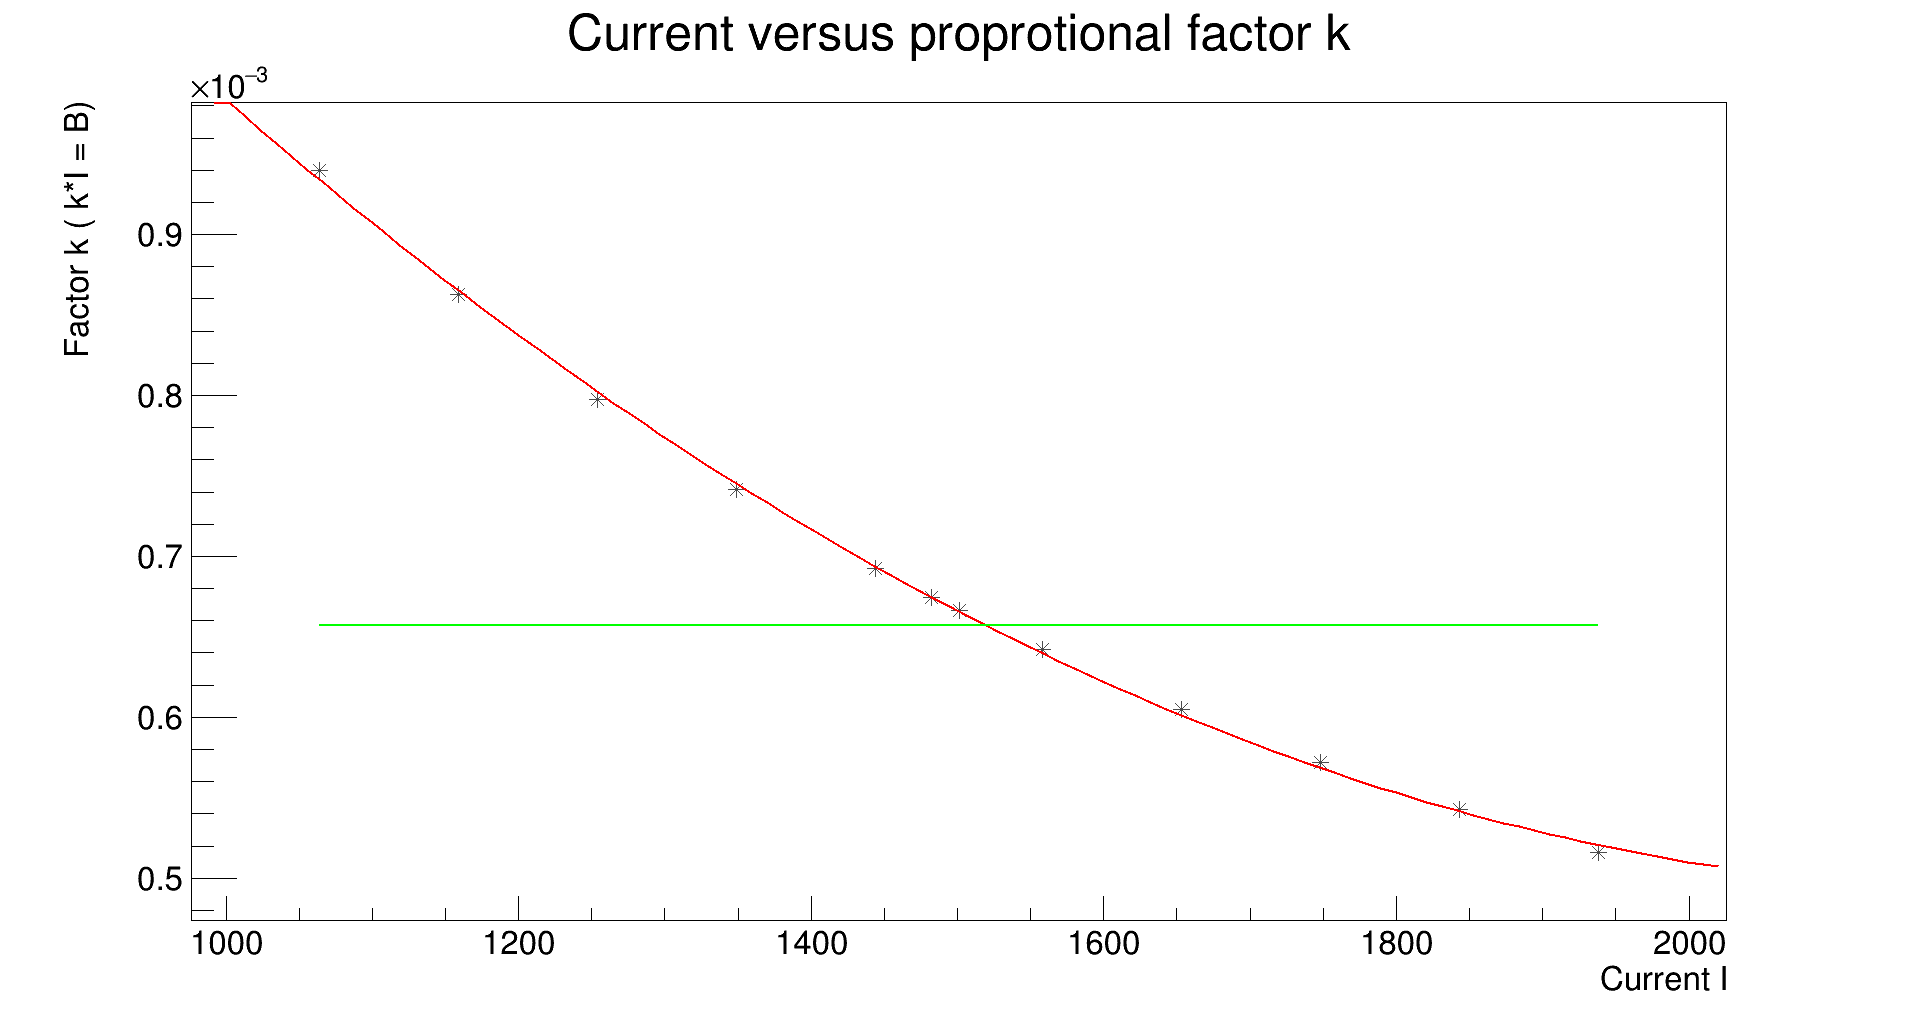
\includegraphics[width=.9\linewidth]{k_pol2.png}
	\caption{"Current vs proportional factor $k$ for RUNs 39-61.Green line: $k$ value from fit B vs I; red line: Fit of $k$ vs I with $ax^{2}+bx +c$ "}
	\label{fig:k_vs_i_pol2}
\end{figure}

\subsection{Plotting ramp up and ramp down separately}
In figure \ref{fig:ramp_up_down} the datapoints for the ramp up (from 1482 Ampere to 1938 Ampere) and ramp down (from 1444 Ampere to 1064) are plotted separately and both fitted with a 3rd order polynomial (a$\cdot$x +b$\cdot x^{2}$ + c$\cdot x^{3}$).
\begin{figure}[!htbp]
	\centering
	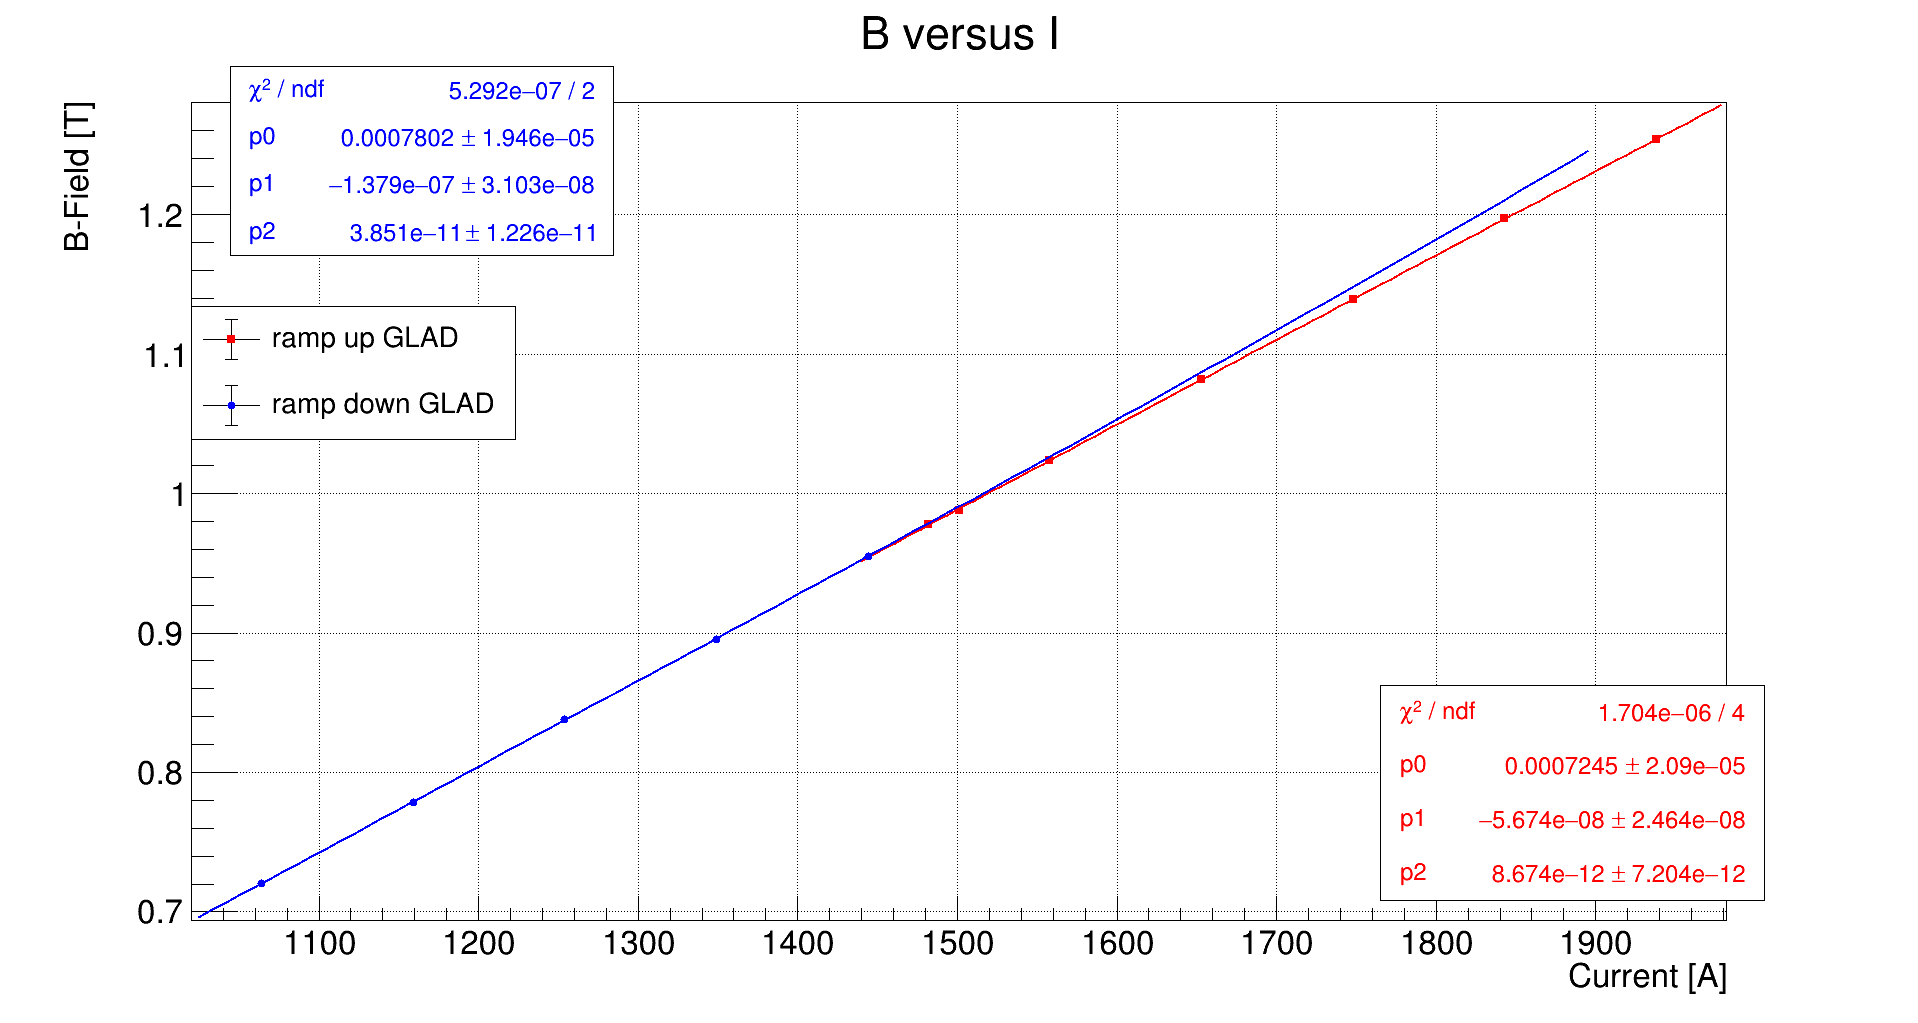
\includegraphics[width=.9\linewidth]{ramp_up_down.png}
	\caption{"B-Field versus current for both ramp up and down phase."}
	\label{fig:ramp_up_down}
\end{figure}

From figure \ref{fig:ramp_up_down} we can see that the slope of the fit for the ramping down phase is steeper as in the ramping up phase. As the current ranges for the two phases don't overlap we cannot derive any other information from the plot. 
\section{Plots with errors in B ( = 6.3472/radius)}
Therefore $\sigma_{B}$ (coming from the error in the radius computation) has to be extracted to get the standard error of the mean (SEM).
\begin{tabular}{|c|c|c|c|}
\hline
Runnr. & B-mean & $\sigma_{B}$ & No. of Events & SEM \\
\hline
39		&

\end{document}
